\documentclass[12pt]{article}
\usepackage{amsfonts}
\usepackage{amsmath}
\usepackage{amsthm}
\usepackage[english]{babel}
\usepackage{booktabs}
\usepackage[labelfont=bf]{caption}
\usepackage{epigraph}
\usepackage{fullpage}
\usepackage{graphicx}
\usepackage[utf8]{inputenc}
\usepackage{nicefrac}
\usepackage[numbers]{natbib}
\usepackage{parskip}
\usepackage{subcaption}

\usepackage[
  colorlinks=true,
  linkcolor=black,
  anchorcolor=black,
  citecolor=black,
  filecolor=black,
  menucolor=black,
  runcolor=black,
  urlcolor=black]{hyperref}

\newtheorem*{definition}{Definition}

\theoremstyle{definition}
\newtheorem{example}{Example}[section]

\DeclareMathOperator*{\argmin}{arg\,min}
\newcommand{\calN}{\mathcal{N}}
\newcommand{\hic}{\textup{HIC}}

\title{Hierarchical Information Content:\\
    Complexity at the Nexus of Order and Disorder}
\author{Awni Hannun\footnote{
  Send correspondence to
  \href{mailto:awni.hannun@gmail.com}{awni.hannun@gmail.com}}}

\date{\today}

\begin{document}
\maketitle

\begin{abstract}
  As simulations of digital life increase in scale, identifying interesting
    emergent structures and processes becomes a challenge.  Solving this will
    require quantitative criteria which align with the goals of the system
    designer. Such criteria are usually reduced to a measure of complexity. We
    argue that complexity growth is induced at the composition of order and
    disorder. Hierarchies built from such compositions lead to further
    increasing complexity. Based on these observations we define
    \emph{hierarchical information content} and motivate it as a measure of
    complexity. We demonstrate with experiments on elementary cellular automata
    that hierarchical information content successfully distinguishes systems
    based on their complexity.
\end{abstract}

\section{Introduction}
\label{sec:intro}

In digital simulations of life the goal is to induce the emergence of certain
structures or processes. These might include self-replicating or autopoietic
organisms, evolutionary processes, and intelligent behavior. Often identifying
the growth of these structures and processes is reduced to identifying a growth
in complexity. Hence designers of artificial life simulations are interested in
the question of measuring complexity.

As artificial life simulations scale, quantitative assessment of the
simulation's success in meeting the designer's criteria is essential.
Identifying and selecting amongst the design choices of a given simulation in a
qualitative manner is not scalable and likely to admit experimental bias. As an
analogy, imagine constructing a machine-learning model to learn a given task
without an objective function. Curiosity driven exploration and reinforcement
learning can result in the model learning to successfully complete the task.
However, from the empiricists perspective, assessing the ability of the model
at completing the task is critical. At the very least, some criterion is needed
for evaluating the model, if not training it. Similarly, in artificial life,
while the measure of complexity is typically not used as an objective to guide
the active simulation, it is at least essential to evaluate the post-hoc
success of the simulation.

Complexity is notoriously ill-defined, subjective, and hence difficult to
measure quantitatively~\citep{gell2002complexity, mitchell2009complexity,
wiesner2019measuring}. One of the challenges in measuring complexity is
identifying the ``Goldilock's zone'' between total order and total disorder
where complexity may reside (\emph{c.f.}
figure~\ref{fig:complexity_and_entropy}). Information theoretic measures such
as Shannon entropy~\citep{shannon1948} and Kolmogorov complexity (sometimes
called Algorithmic Information Content)~\citep{kolmogorov1965, solomonoff1964},
are actually measures of randomness. As figure~\ref{fig:complexity_and_entropy}
illustrates, these measures increase monotonically with the disorder of a
system.

\begin{figure}
\centering
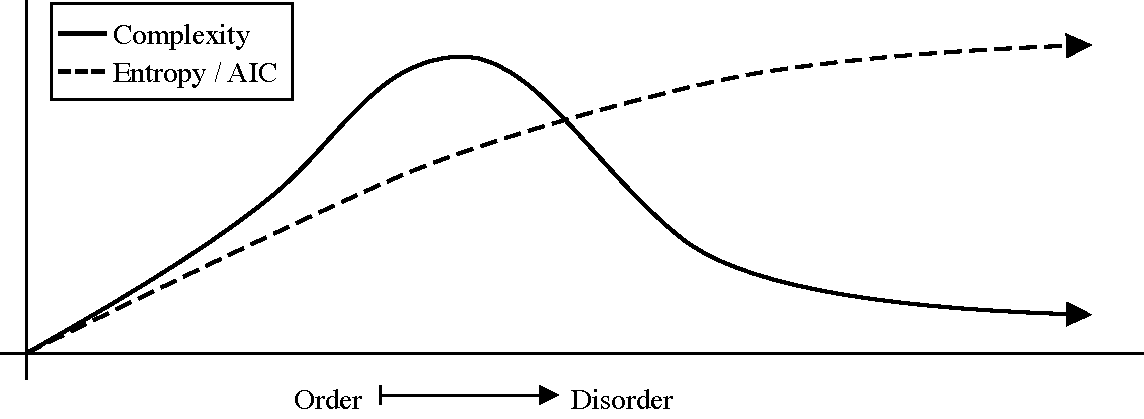
\includegraphics[width=0.7\textwidth]{figures/complexity_and_entropy}
\caption{TODO}
\label{fig:complexity_and_entropy}
\end{figure}

Because of this difficulty, many measures of complexity have been
proposed~\citep{lloyd2001measures}, all with differing trade-offs. Often they
fail the ``one-hump'' criterion~\citep{adami2002complexity} increasing with
order or disorder. This is typical of the aforementioned information theoretic
criteria (Shannon entropy and Kolmogorov complexity) and constructions which
use them~\citep{lloyd1988complexity}. Other measures which satisfy the one-hump
test are not easily made operational requiring either a large degree of
subjective input from the designer or are exceedingly difficult to
compute~\citep{crutchfield1989inferring, gell1996information,
grassberger1986toward}.

We propose yet another a measure complexity, Hierarchical Information Content
(HIC). The central tenent of HIC is that complexity growth is found at the
compositions of ordered and disordered systems. We elaborate and defend the
motivating princpiles of HIC in section~\ref{sec:finding_complexity}. We do not
intend for HIC to serve as an ersatz for complexity in a general sense, and in
fact we make make no further attempt to rigorously define complexity. Rather,
we propose HIC as a measure which quantitatively captures some of the essential
aspects of complex systems. We promptly disclose two limitations of HIC. First,
HIC is not intended to work well for every case, but to work well for many
cases that are of interest, particularly in simulations of artificial life.
Second, while HIC can be used with few assumptions, in many instances it may
gain utility from the subjective input by the designer of the system.

\section{Finding Complexity}
\label{sec:finding_complexity}

We hypothesize that complexity grows from the compositions of order and
disorder.  When a system composes an ordered structure a disordered collection of 
subsystems, opportunity for complexity growth emerges. At a higher level many
ordered structures can become disordered. This leads to a hierarchy of levels
with varying degrees of order and disorder creating a complex macro structure.
We motivate the idea of inducing complexity from composing order and disorder
in the sequel, followed by a motivation of the importance of hierarchies. 

\subsection{Order and Disorder}

\citet{adami2002complexity} define two types of complexity: i) \emph{structural
complexity}, which can be thought of as complexity in space and ii)
\emph{process complexity}, which can be thought of as complexity in time.
Following \citet{schrodinger1944}, we consider two types of composition. The
first is order from order, and the second is order from disorder.  \citet[chap.
6]{schrodinger1944} argues that living beings exhibit order from order. In an
abstract sense, a living organism ``feeds on negative entropy'' (\emph{i.e.}
order) to produce the necessary building blocks needed to reduce the organisms
natural tendency towards entropy. More concretely, organisms create highly
structured subsystems at the molecular level (DNA, RNA, proteins, \emph{etc.})
by metabolising highly structured inputs. This process describes the
development of complexity through time. Hence complexity in time (process
complexity) involves the composition of order from order. 

On the otherhand, complexity in space constructs higher-level structures from
lower level structures. If the structures are ordered throughout the levels of
the hierarchy, the global structure is unlikely to be complex. Some degree of
disorder should be present at various levels of the hierarchy. Thus complexity
in space (structural complexity) emerges in part from the composition of order
from disorder.

Given the distinctions between how complexity manifests in time and space two
separate measures may be appropriate. Here, we are solely concerned with the
later -- measuring complexity in space. The nexus of complexity growth in space
is found in the composition of order from disorder. In order to continue to
grow complexity a structure must continue to increase the number of such
compositions. A hierarchy must develop where some levels are more ordered and
some are more disorderd. This is the primary motivation of our measure of
complexity which we define more rigorously in section~\ref{sec:hic}.

\subsection{Hierarchical Systems and Complexity}

Many complex systems found in nature, both biotic and abiotic, have a
hierarchical structure. For example, the hierarchical structure of a cell
proceeds from atoms to molecules, then marcomolecules, then
organelles. Cells themselves aggregate into multicellular constructs which form
organs which result in human beings. Social systems almost always have
hierarchical structure. A complex business consists of individual workers,
teams, departments, business units, subsidiaries, and finally the company itself.
The abiotic galactic system is structured as a hierarchy consisting of
planets, solar systems, star clusters, galaxies, and even galactic clusters.

Following \citet{simon1991architecture}, we give an explanation for why complex
systems in nature are much more likely to be hierarchical than not. Emergent
and stable structure must develop much faster than the rate of detioration
driven by the second law of thermodynamics. A small number of detiorations can
cause a catastrophic failure which means the assembly process must begin from
scratch.  Hence, an attempt to assemble a complex structure \emph{de novo}
which is stable only upon completion is unlikely to succeed. Rather, a
hierachical assembly through intermediate stepping stones of stable subsystems
is more likely to result in the succesful assembly of the full system. If at
any stage a detioration occurs, the assembly need not start from scratch but
can draw on existing already assembled subsystems. The stable subsystems can be
assembled quickly from their own constituent susbsytems, so they too are less
likely to be thwarted by increasing entropy. The subsystems can be used to
rapidly assemble a larger more complex stable system.

In a related argument, \citet{cairns1995complexity} argues that since evolution
proceeds by small mutations a scaffold of sorts is required to develop complex
structures. Once the complex structure is functional (\emph{i.e.} provides a
reproductive benefit), the scaffold can be lost without harm. With the
scaffold lost, evolution must proceed in a forward, complexity increasing
direction to further optimize an organism in a given niche. This so-called
``complexity ratchet'' gives both a mechanism to enable complexity growth and
an explanation for why the growth appears to be monotonic. In terms of
hierarchical structure, the scaffolding can be thought of as a structure which
holds together subsystems. When a reproductive advantage emerges from the
combination of the subsystems, the scaffolding can fall away resulting in a
more complex and hierarchical structure.

The process of using subsystems to create more complex larger systems is well
documented in evolution and the history of life. For example most of the
``major transitions''\footnote{These include the compartmentalization of
molecules, the hypothesized aggregation of RNA into Chromosomes, the
hypothesized symbiosis of two Prokaryotic cells into the Eukaryotic cell,
unicellular to multicellular organisms, individuals to colonies, and small
human groups to human societies.} in the evolution of life involve the
construction of a higher-level organism from lower level
components~\citep{smith1997major}. Using the fossil record as evidence,
\citet{mcshea2001hierarchical} demonstrates an increase in the maximum
hierarchical structure (the number of nested levels) found in organisms over
the course of evolution.\footnote{Curiously \citet{mcshea2001hierarchical} also
finds evidence for an increase in the rate of increase in the maximum
hierarchical structure. An optimistic implication is that an increase in
hierarchical complexity leads to an increase in the evolvability of an
organism.}  

Complexity via composition and hierarchy has been demonstrated in simulations
of artificial chemistries~\citep{rasmussen2001ansatz, sayama2019cardinality}.
\citet{rasmussen2001ansatz} state as an ansatz that a sufficiently
complex set of subsystems is both necessary and sufficient for hierarchical
complexity to emerge. \citet{sayama2019cardinality} suggests that the
composition of lower-level primitives into higher-level structure results in a
``cardinality leap''. A finite set of building blocks can yield a countably
infinite set of higher-level structures. This provides an explanation for why
higher-level structure can be correlated with an increase in complexity,
particularly in the presence of natural selection.

\section{Hierarchical Information Content}
\label{sec:hic}

We construct a measure for the structural complexity of a system. As motivated
in section~\ref{}, the complexity should grow through the compositions of
ordered and disordered subsystems in a hierarchical structure. At each such
composition (whether it by order to disorder or disorder to order), the
complexity grows. Hence we decompose the overall complexity as the sum of the
complexity at each such composition.

The complexity at each composition is given by the difference in mutual
information between the higher-level system and that of the subsystem. We
denote by $X^{\ell}$ the state variable at the $\ell$-th level of the
hierarchy. The neighborhood of $X^\ell$ is the set $\calN(X^\ell)$ which
contains the elements used to construct the system at the next level. Following
\citet{simon1991architecture}, we define the span of a level $d^\ell =
\left|\calN(X^\ell)\right|$ as the number of elements in the neighborhood. For
now we assume the span to be constant with a value of two $d^\ell = 2$ for
every level. We later generalize to larger spans.

The complexity at the composition of level $\ell$ from level $\ell -1$ is
computed from the squared difference of the mutual information of the
neighborhood at each level:
\begin{equation}
  C_\ell = \left[ I(X^{\ell+1}; Y^{\ell+1}) - I(X^\ell; Y^\ell) \right]^2
\end{equation}
The mutual information can be computed from the Shannon entropy and conditional
entropy when $X^\ell$ is discrete or the differential entropy when $X^\ell$ is
continuous~\citep{cover1999elements}:
\begin{equation}
\label{eq:mutual_information}
I(X^\ell; Y^\ell) = H(X^\ell) - H(X^\ell \mid Y^\ell)
\end{equation}

We use the level complexities $C_\ell$ to construct the overall system complexity.
\begin{definition}[Hierarchical Information Content]
\label{def:hic}
  The Hierarchical Information Content (HIC) of a hierarchical system $S$ with
  $L$ levels is given by:
  \begin{equation}
    \label{eq:hic}
    \hic(S) = \sum_{l=1}^{L-1} C_\ell = \sum_{l=1}^{L-1} \left[ I(X^{\ell+1}; Y^{\ell+1}) - I(X^\ell; Y^\ell) \right]^2.
  \end{equation}
\end{definition}

\subsection{Examples}

We attempt to build intuition for the definition of HIC through some simple
examples.

\begin{example}
  \label{ex:constant}
  As a first example, consider a state $S = [0, 0, \ldots, 0]$,
  constant sequence of all $0$s. At any level for any neighborhood, the mutual
  information $I(X^\ell; Y^\ell) = 0$. Hence the terms $C_\ell = 0$ for all
  $\ell$ and the overall $\hic(S) = 0$.
\end{example}

\begin{example}
  \label{ex:uniform}
  Let $S = [x_1, x_2, \ldots]$ consist of a sequence of independent draws from a
  multinomial uniform distribution over $K$ categories. Assuming a span of $2$,
  the variable $X^\ell$ consists of $2^\ell$ of the $x_i$ prmitives and hence
  can take on any of $K^(2^\ell)$ values. Consider the mutual information level
  $\ell$:
  \begin{equation}
    I(X^\ell; Y^\ell) = H(X^\ell) - H(X^\ell \mid Y^{\ell}) = 2^\ell \log K - 2^\ell \log K = 0
  \end{equation}
  Hence all of the $C^\ell = 0$ and $\hic(S) = 0$.
\end{example}

As examples~\ref{ex:constant} and \ref{ex:uniform} show, HIC behaves as
expected when the system exhibits complete order or complete disorder. In both
of these examples the HIC was zero because all of the mutual informations were
themselves zero. In the following example, we see slightly more interesting
behavior, where the individual mutual informations are not zero, but the
resulting HIC is.

\begin{example}
  \label{ex:repeats}
  Let $S = [0, 1, 0, 1, \ldots]$ consist of a sequence of alternating zeros and
  ones.

  For the first level $X^1$ takes on the two values $\{0, 1\}$ with equal
  probability hence $H(X^1) = \log 2$. However given the neighbor $Y^1$ the
  value of $X^1$ is deterministic and hence $H(X^1 \mid Y^1) = 0$. Thus the
  overall mutual information is $I(X^1; Y^1) = \log 2$.

  For the second level $X^2$ takes on two values $\{[0, 1], [1, 0]\}$ with
  equal probability, and we have $H(X^2) = \log 2$. Again $X^2$ is fully
  determined by $Y^2$ thus $H(X^2 \mid Y^2) = 0$ and $I(X^2, Y^2) = \log 2$.
  Combining these to produce $C^2$ yields:
  \begin{equation}
    C^2 = (I(X^2; Y^2) - I(X^1; Y^1))^2 = (\log 2 - \log 2)^2 = 0.
  \end{equation}
  The above argument generalizes to all $\ell$ so $\hic(S) = 0$.
\end{example}

In example \ref{ex:repeats} we used overlaping windows to construct $X^2$. If
had chosen disjoint windows the HIC would be small but nonzero. Depending on
the problem this may be desirable in that the alternating seuqence should be
considered slightly more complex than a constant sequence. This is where
subjectivitity comes in. The designer should determine among these choices
based on the setting at hand.

\begin{figure}[ht]
\centering
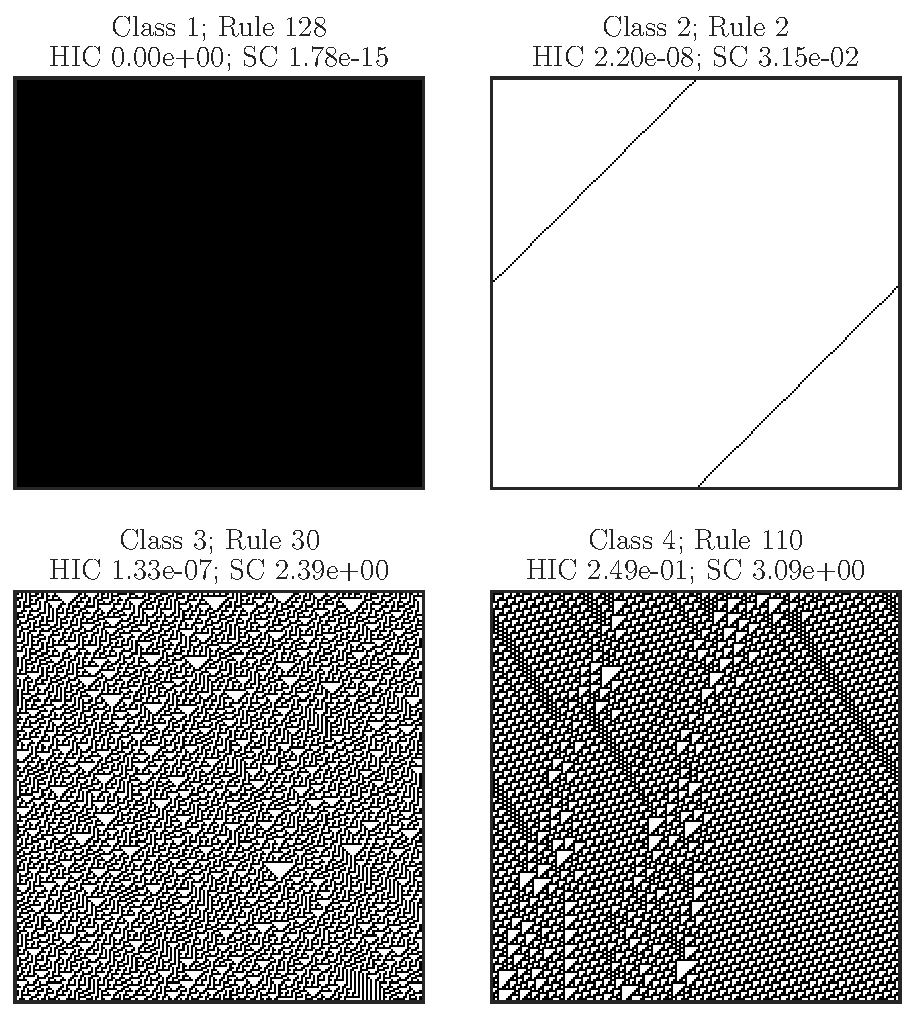
\includegraphics[width=0.7\textwidth]{figures/eca_images_and_complexity}
\caption{Example ECA rules from the four Wolfram classes. Each ECA has a state
    size of $N=200$ states and is run for $400$ steps. The latter $200$ steps
    are visualized above. We compute the HIC for each ECA using $L=3$ levels.}
\label{fig:eca_images_and_complexity}
\end{figure}

\section{Experiments}

\subsection{Experimental Setting}

We examine HIC empirically using elementary cellular automata (ECA). We also
compare HIC to statistical complexity for varioius ECA. Cells in an ECA
can take on one of two states. The update rule for a given state depends on the
state at the previous time step along with its two neighbors; hence there are
$2^{(2^3)} = 256$ possible ECAs. \citet{wolfram1983} proposed a four class
system to categorize ECA rules by their typical behavior. Class 1 ECAs converge
to a constant state, class 2 ECAs tend to exhibit periodic oscillations, class
3 ECAs display random-like behavior, and class 4 ECAs show complex behavior.
Complex behavior of an ECA is not well defined and is determined mostly through
inspection. The complex ECAs usually have various high-level structures
propagating through time with some degree of apparant randomness interspersed
between. Despite the simplicity of the rules, ECAs can yield astonishingly
complex behavior. Rule 110, for example, has been shown to be computationally
universal~\citep{cook2004universality}. We follow the Wolfram classification
given by~\citet[table 2]{martinez2013note} to classify all 256 ECA rules.

For each ECA we use a state size of $N$. The information in the initial state
requires at least $N/2$ updates to propagate accross the complete state space.
We update the ECA for $2N$ time steps and discard the first $N$ which provides
a buffer for information in the initial state to fully propagate. We use a
circular update so the cells at the edges are influenced by neighbors at the
opposite edge of the state.  Because of this, rules which propagate information
unidirectionaly can influence the full state space after $N$ updates.

We use the remaining $N \times N$ cells to compute the HIC. At each level we
set $X^\ell$ and $Y^\ell$, the variables used to compute the mutual information
in equation~\ref{eq:mutual_information}, to be neighboring sequences each
consisting of $\ell$ cells. So for the first level ($\ell = 1$) $X$ and $Y$ are
single and consecutive cells, for $\ell = 2$ the variables are consecutive but
disjoint pairs of cells, and so on. We estimate the distributions $P(X^\ell)$
and $P(X^\ell \mid Y^\ell)$ used to compute the mutual information at each
level from counts over the states.

To construct the causal states for statistical complexity, we use the
Kullback-Leibler divergence with a threshold of $1.0$. We use a past light cone
with $T_{\textrm{P}}=2$ and a future light cone with $T_{\textrm{F}} = 3$.  For
each time step the number of states in the light cone grows by two. For
example, the third time step of the future light cone contains five cells. As
with HIC we esimtate the distributions using counts over the states.

\begin{figure}[ht!]
\centering
\begin{subfigure}{\textwidth}
    \centering
    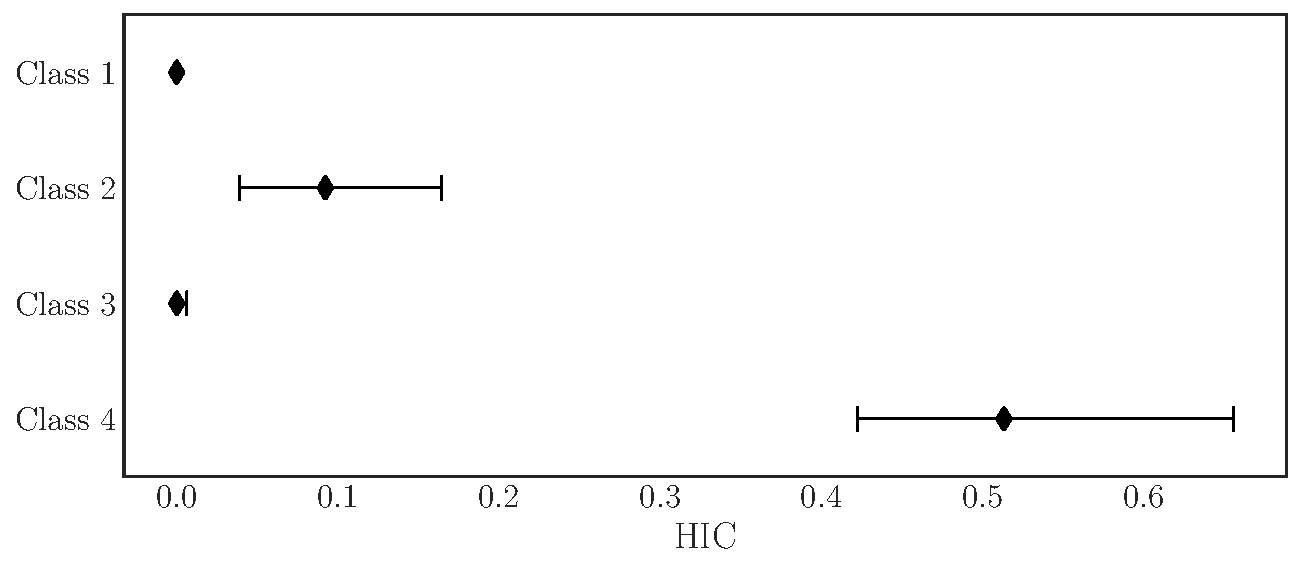
\includegraphics[width=0.8\textwidth]{figures/hic_by_class}
    \caption{Hierarchical information content (HIC)}
    \label{fig:hic_by_class}
\end{subfigure}
\begin{subfigure}{\textwidth}
    \centering
    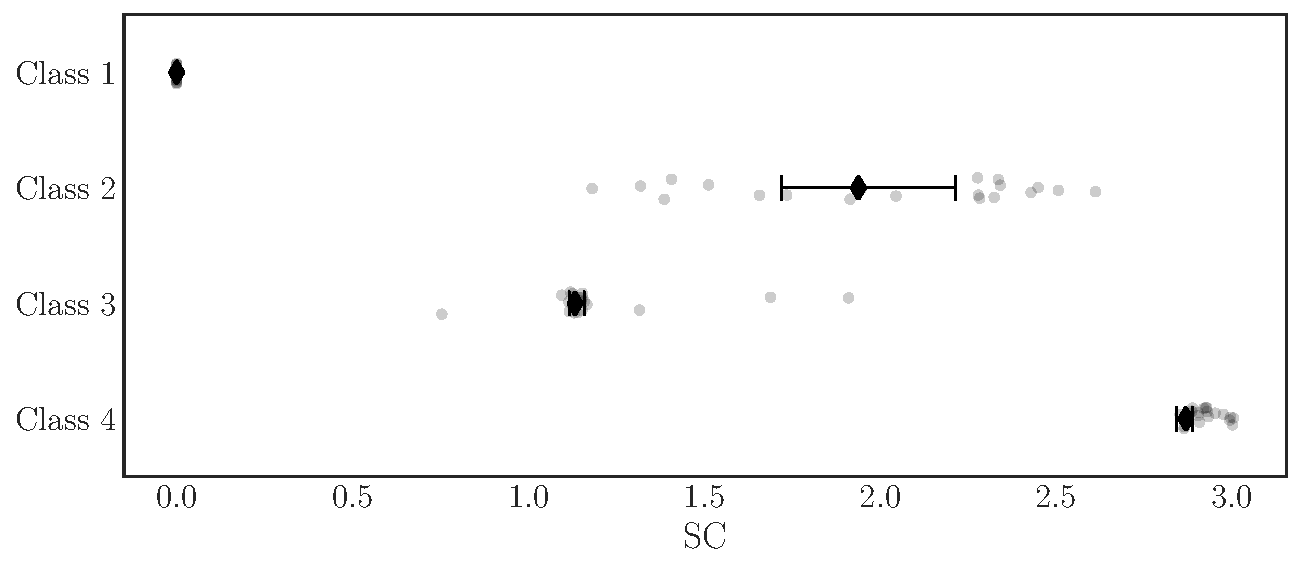
\includegraphics[width=0.8\textwidth]{figures/sc_by_class}
    \caption{Statistical complexity (SC)}
    \label{fig:sc_by_class}
\end{subfigure}
\caption{The median and 95\% confidence intervals for the HIC for each Wolfram
    class. We compute these by randomly sampling 100 rules with random initial
    states and computing the HIC of each. For each class, the first twenty
    trials within one standard deviation of the median are plotted.}
\label{fig:complexity_by_class}
\end{figure}


\subsection{Comparing HIC to Statistical Complexity}

Figure~\ref{fig:eca_images_and_complexity} shows a canonical ECA rule from each
class: rule 128 is class 1, rule 2 is class 2, rule 30 is class 3, and rule 110
is class 4. For these simulations we use $N\!=\!200$ and an initial state of all
inactive cells (zeros) with a single active cell (one) at the center. We
compute the HIC over $L\!=\!3$ levels. The HIC is given for each rule above the
corresponding image. Note that HIC correctly distinguishes rule 110 as being
the most complex ECA from the remainder, which have HICs very close to zero.
Note in particular that the HIC of the class 3 ECA (rule 30) is even smaller
than the corresponding class 2 ECA (rule 2). In this case HIC peaks inbetween
order and disorder, as desired. We also see that the statistical complexity
(SC) correctly orders the rules from each class. However, unlike HIC the class
3 ECA (rule 30) has a fairly large statistical complexity. This is the case
because the ECA exhibits randomness over the spatial dimension but has some
structure over the temporal dimensions.

Figure~\ref{fig:complexity_by_class} demonstrates that both HIC and statistical
complexity can distinguish between the four Wolfram complexity classes. These
results are obtained by sampling $100$ rules for each of the four ECA classes.
Each rule is run from a random initial state for $1000$ steps. We use a state
size of $N\!=\!500$ and hence a $500 \times 500$ grid to compute the
corresponding complexity measure. For these experiments we use $L=6$ levels for
the HIC. The class medians are well separated by the median HIC
(fig.~\ref{fig:hic_by_class}) with the 95\% confidence interval of class 4
distinct from that of any other class.

We also plot in figure~\ref{fig:hic_by_class} the first twenty trials for each
class with an HIC within one standard deviation of the median. Rules from ECA
class 2 have the widest range of HIC. Qualitative inspection of the high HIC
results shows many cases where the resulting state is simply shifted to the
left or right by the rule. The state exhibits a simple periodic pattern over
time but because of the random initialization, the pattern over space does not
appear to be simple. This is one failure mode of HIC -- it does not
capture the simplicity over the time dimension given that it is only applied to
the space dimension.

The statistical complexity medians are less well separated than those computed
from the HIC. On the other hand, the statistical complexity
(fig.~\ref{fig:sc_by_class}) has narrower 95\% confidence intervals for all
classes. Overall, both measures are quite good at distinguish complex class 4
ECA from the rest. Both measures could be useful depending on whether one
intends to measure process or structural complexity. The two may also be
combined to produce a single more comprehensive measure.

\subsection{Number of Levels}

\begin{figure}[t]
\centering
\begin{subfigure}{0.45\textwidth}
  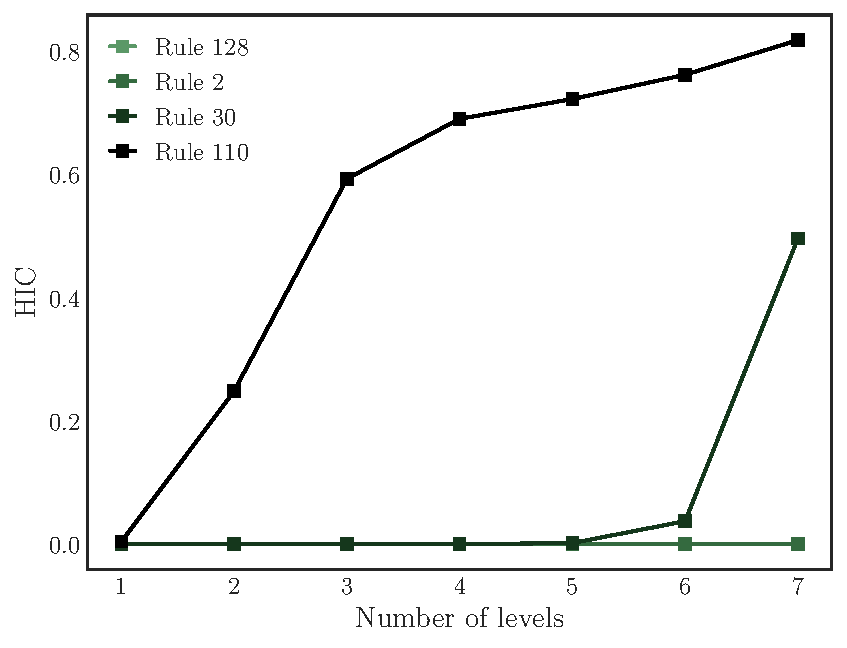
\includegraphics[width=1.0\textwidth]{figures/hic_vs_num_levels_size_200}
  \caption{State size $N = 200$}
  \label{fig:hic_levels_200}
\end{subfigure}
\begin{subfigure}{0.45\textwidth}
  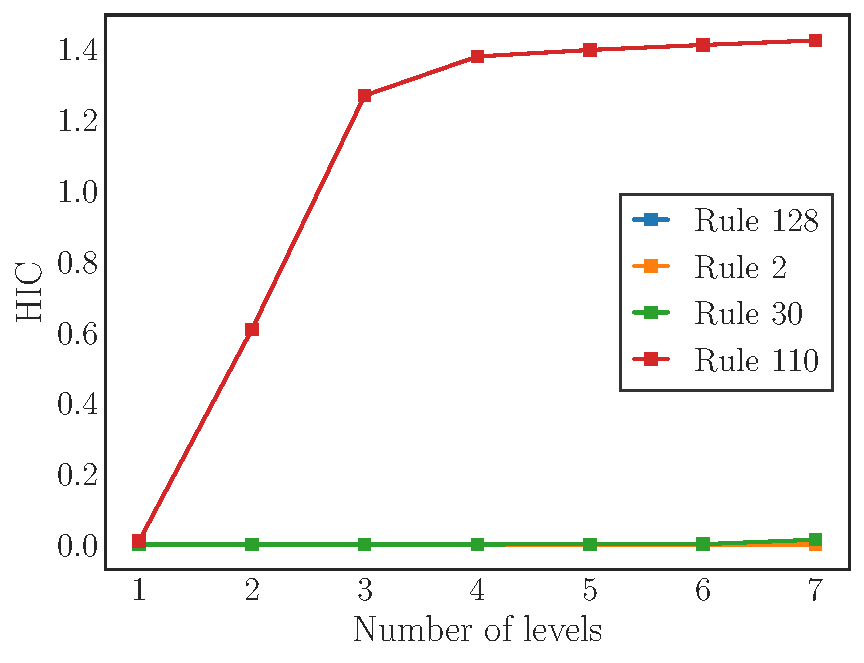
\includegraphics[width=1.0\textwidth]{figures/hic_vs_num_levels_size_500}
  \caption{State size $N = 500$}
  \label{fig:hic_levels_500}
\end{subfigure}
\caption{We show the HIC versus the number of levels $L$ used in the
    computation. We compute the HIC for one rule from each of the four Wolfram
    classes. Each ECA is run for $2N$ time steps and the HIC is computed from
    the latter half.}
\label{fig:hic_vs_levels}
\end{figure}

Using the same four rules (class 1 rule 128, class 2 rule 2, class 3 rule 30
and class 4 rule 110), we observe the effect of the number of levels on the HIC
in figure~\ref{fig:hic_vs_levels}. Figure~\ref{fig:hic_levels_200} uses a state
size of $N\!=\!200$, and figure~\ref{fig:hic_levels_500} uses a state size of
$N\!=\!500$. In both figures, we see that the class 1 and 2 rules (the curves
overlap at zero) do not grow with an increase in the number of levels. The
class 4 rule grows but plateaus with the number of levels. We expect to see a
plateau once the size of the variables $X^\ell$ and $Y^\ell$ fully capture the
the largest structures, and so the mutual information should become constant.
This shows that complexity does not grow via compositions of order from order.
Interposing disorder somewhere near the level of the largest structures would
result in further complexity growth.

The class 3 ECA is the only one which exhibits a qualitative difference between
the two figures. This is simply a finite sample statistical artifact which is
instuctive to elucidate. In the $N\!=\!200$ case, we do not have enough states to
estimate the mutual information at the highest level ($\ell\!=\!7$) accurately.
The mutual information consists of two terms, the entropy of the single
variable $H(X^\ell)$ and the conditional entropy between the two variables
$H(X^\ell \mid Y^\ell)$. The entropy requires fewer samples to estimate
accurately than the conditional entropy. For example $X^7$ can take on $2^7$
possible values whereas the pair $(X^7, Y^7)$ admits $2^{14}$ distinct values.
With insufficient sample sizes, the conditional entropy shrinks prior to the
entropy and the mutual information is artificially inflated. This can be
remedied by increasing $N$. However, a parametric or otherwise more sample
efficient model for $P(X)$ and $P(X \mid Y)$ is an alternative that will likely
scale more robustly with the number of values of $X^\ell$.

\section{Discussion}

As simulations of digital life scale, robust and easy to implement measures
which can automatically detect emergent complexity will be critical.
Hierarchical information content is one such measure which can distinguish
systems with structural complexity from both purely random and highly ordered
systems. In other words, HIC exhibits the single hump in between order and
disorder required of any useful measure of complexity (see
fig.~\ref{fig:complexity_and_entropy}).

One of the benefits of HIC over some alternative measures of complexity is that
it requires very few assumptions to be used with a system. At most the levels
of the system and the sub-modules which make up a given level must be
determined. For systems which exhibit a natural hierarchy, HIC can be deployed
directly. We argued in section~\ref{sec:hierarchy_and_complexity} that
hierarchical structure drives complexity growth, and hence many naturally
occurring complex systems are hierarchical.

We've shown that HIC can distinguish complex elementary cellular automata from
random and highly ordered ones. Further studies should validate that HIC can
distinguish complexity in other artificial and natural systems. For example we
aim to apply HIC to two-dimensional cellular automata and to artificial
chemistries. We also intend to observe how well HIC captures the complexity of
natural systems, including for example protein networks or DNA sequences.

In many cases HIC on its own is sufficient, particularly when a system exhibits
a natural hierarchy and when measuring process complexity is not important.
However, we encourage researchers to consider HIC as one more tool in the
complexity measuring toolkit. For example, HIC and statistical complexity
together could capture both process and structural complexity which would be
difficult for either to capture when used in isolation.

Ultimately any purely quantitative measure of complexity should be used
carefully. Often objective functions that can be optimized numerically are
proxies for the intended goal. Prior to using a proxy one must validate that it
does indeed correlate with the intended goal. In the same way HIC, and any
other measure of complexity, should be validated prior to use with any new
system. Removing all subjectivity in assessing the complexity of a system is
difficult. A system which appears random to one observer can be meaningful
to another in the same way that the interpretation of a string of bits
depends on the recipient. In these cases, encoding prior information about the
structure of the system in the states used to compute the HIC will make it more
useful as a measure of complexity.

\citet[chap. 23]{hamming1997art} correctly predicted that ``we will...want
Mathematical models in which the whole is not the sum of the parts, but the
whole may be much more due to the `synergism' between the parts''. We are still
at the beginning of understanding the nature of complexity particularly as it
emerges from the interaction of simpler subsystems. Our understanding of
complex systems will grow through the use of tools like hierarchical
information content and other measures of complexity. We hope this will put
researchers in a better position in the future to formulate a more unified
theory of complexity.


\bibliographystyle{plainnat}
\bibliography{references}

\end{document}
